\chapter{Diseño e implementación de los sistemas SL y SL mini}

En este capítulo se realizará una explicación del diseño de los sistemas SL y SL mini, analizando las diferentes alternativas de placas, junto con sensores seleccionados y el modelado en 3D de la caja que alojará los mismos. Por último se detallará la implementación de los drivers escritos en Python 3, considerando elecciones de diseño.

\section{Análisis de requisitos}

Para definir algunos requerimientos es necesario evaluar las alternativas existen en el mercado de sistemas de acceso vehicular, y proponer un sistema capaz de suplir las desventajas o mejorar ventajas para los usuarios.

\subsection{Sistemas actuales}

Los sistemas actuales más comunes hoy en día son:

\subsubsection{Sistemas tradicionales de tickets}

Este sistema de control de ingreso y egreso suele generar molestias en muchos de los usuarios, por la necesidad de realizar alguna acción extra, como presionar un pulsador para obtener un ticket con los datos de entrada. Este sistema se puede apreciar en Fig. \ref{fig:sistema-tradicional}.
Los tickets poseen un gran inconveniente, ya que si el usuario lo pierde se le cobra un valor fijo que, en general, es mayor al tiempo de la estadía.
Estos sistemas cuentan con el inconveniente de que la impresión del ticket se realiza por impresión térmica, lo que requiere un papel termosensible.
Además, la emisión de papel de un solo uso genera un impacto ambiental a tener en cuenta.
En promedio un usuario tarda 11 segundos en entrar o salir del establecimiento \cite{casadomo_sistema_2015}.

A continuación se resumen las desventajas de este sistema:

\begin{enumerate}
    \item Tiempo de acceso.
    \item Emisión de papeles de un solo uso.
    \item Necesidad de acciones por parte del usuario.
\end{enumerate}

\begin{figure}[bth]
    \centering
    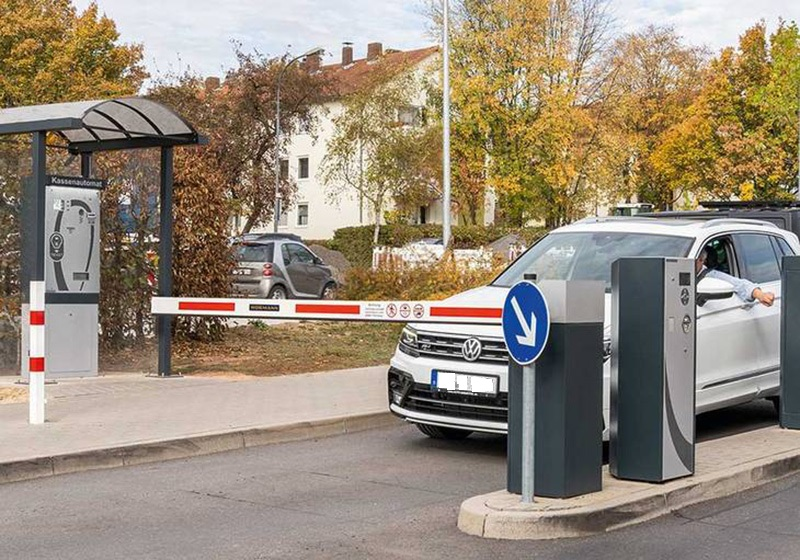
\includegraphics[width=0.5\textwidth]{imgs/sistema-control-acceso-barreras.jpg}
    \caption{Sistema tradicional de acceso por barreras \cite{integralia_sistema_2019}.}
    \label{fig:sistema-tradicional}
\end{figure}

\subsubsection{Sistemas de radiofrecuencia}

Con el avance y el abaratamiento de los costos en la electrónica surgieron nuevos métodos que permitieron a los usuarios prescindir de la necesidad de un ticket o una persona que les permita el acceso. El método principal es el uso de controles remotos que al ser accionados, activan el mecanismo y abren el paso del vehículo.

Otro sistema que está ocupando gran parte del mercado en los últimos años es el que integra a la barrera un sistema de identificador de radiofrecuencia o RFID, que se puede implementar usando de radiofrecuencia (RF) en el vehículo, tarjetas o llaveros RF. Además es necesario instalar un receptor RF en la entrada para producir el enlace y permitir el acceso.
La gran desventaja de este sistema es tener que instalar un emisor RF por cada vehículo o guardar la tarjeta de lectura.

Los problemas de este sistema son:

\begin{enumerate}
    \item Necesidad de instalar un recetor de RF en los puntos de acceso.
    \item Instalar un emisor RF por cada vehículo.
\end{enumerate}

\begin{figure}[bth]
    \centering
    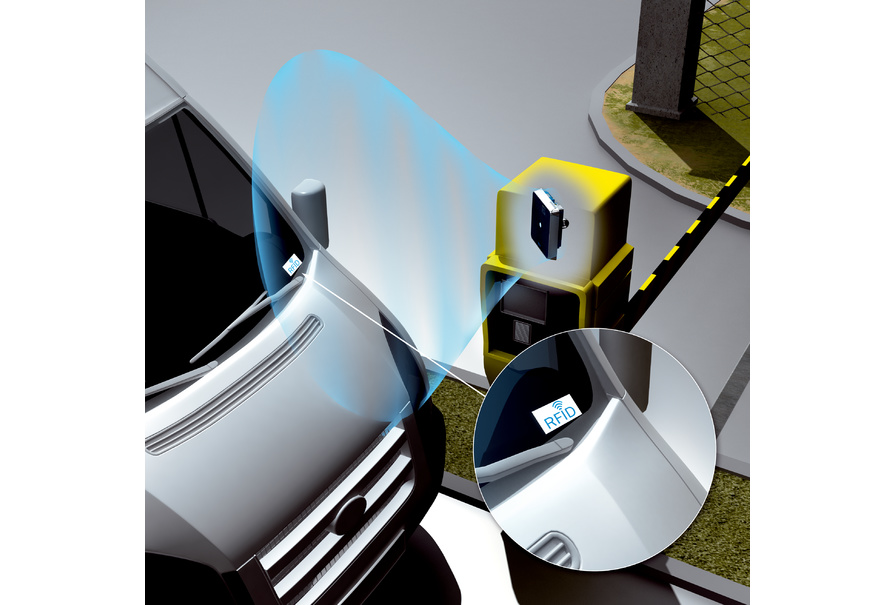
\includegraphics[width=0.8\textwidth]{imgs/sistema-control-acceso-barreras-rfid.jpg}
    \caption{Sistema de acceso por RFID \cite{noauthor_acceso_nodate}.}
    \label{fig:sistema-moderno}
\end{figure}

\subsection{Requisitos de los sistemas SL}

Los métodos anteriormente nombrados son muy útiles en el día a día, pero cuentan con una serie de inconvenientes que pueden ser atenuados mediante el OCR como el descrito en el capítulo 3.
Dicha técnica utiliza un distintivo único de cada vehículo, como en el sistema de RFID, pero la distancia de actuación está dada por la distancia máxima de reconocimiento del algoritmo y los sensores empleados.

Debido a la necesidad de realizar OCR, se requerirá una cámara. Con la finalidad de poder acoplar algún sistema de activación para la cámara se exigirá que la placa elegida soporte protocolos como I2C, SPI y UART. En cuanto a la comunicación, como se implementara junto con un servidor web existe la necesidad de conexión Ethernet o Wifi. Finalmente para facilitar futuras actualizaciones se requiere que la placa pueda correr un sistema operativo basado en GNU/Linux.

En resumen los requerimientos son:

\begin{enumerate}
    \item Colocación de una cámara.
    \item Soporte a protocolos I2C, SPI, UART.
    \item Conexión Ethernet o Wifi.
    \item Tiempo de acceso menor a 11 segundos.
    \item Sistema operativo basado en GNU/Linux.
\end{enumerate}


\section{Selección de placas}

Teniendo en cuenta los requisitos planteados en la sección anterior se presentan varias opciones posibles:
placas de la empresa Raspberry Pi, embebidos de la serie STM32, NVIDIA Jetson e incluso placas de la marca Arduino en sus versiones más potentes, por nombrar las más conocidas.
Aquí es donde surge el primer inconveniente para tomar la elección de placa,
cuál sería la mejor opción que cumpla tanto las necesidades y que sea accesible para poder realizar el proyecto.
Luego de realizar una investigación de placas a las que se podía acceder se optó por dos modelos: uno basado en Raspberry Pi 3 B+ a la cual se la llamó SL mini, y el otro basado en NVIDIA Jetson TX1 denominada SL.

\subsection{Características del SL mini}

La placa del SL mini es una Raspberry Pi 3 B+ \cite{noauthor_documentacion_nodate-2}, Fig. \ref{fig:raspberry} la cual cuenta con un procesador
Broadcom BCM2837B0 y un Córtex A53 acompañado de 1 GB de RAM LPDDR2, junto con un sistema operativo llamado Raspberry Pi OS el cual está basado en Debian.

\begin{figure}[bth]
    \centering
    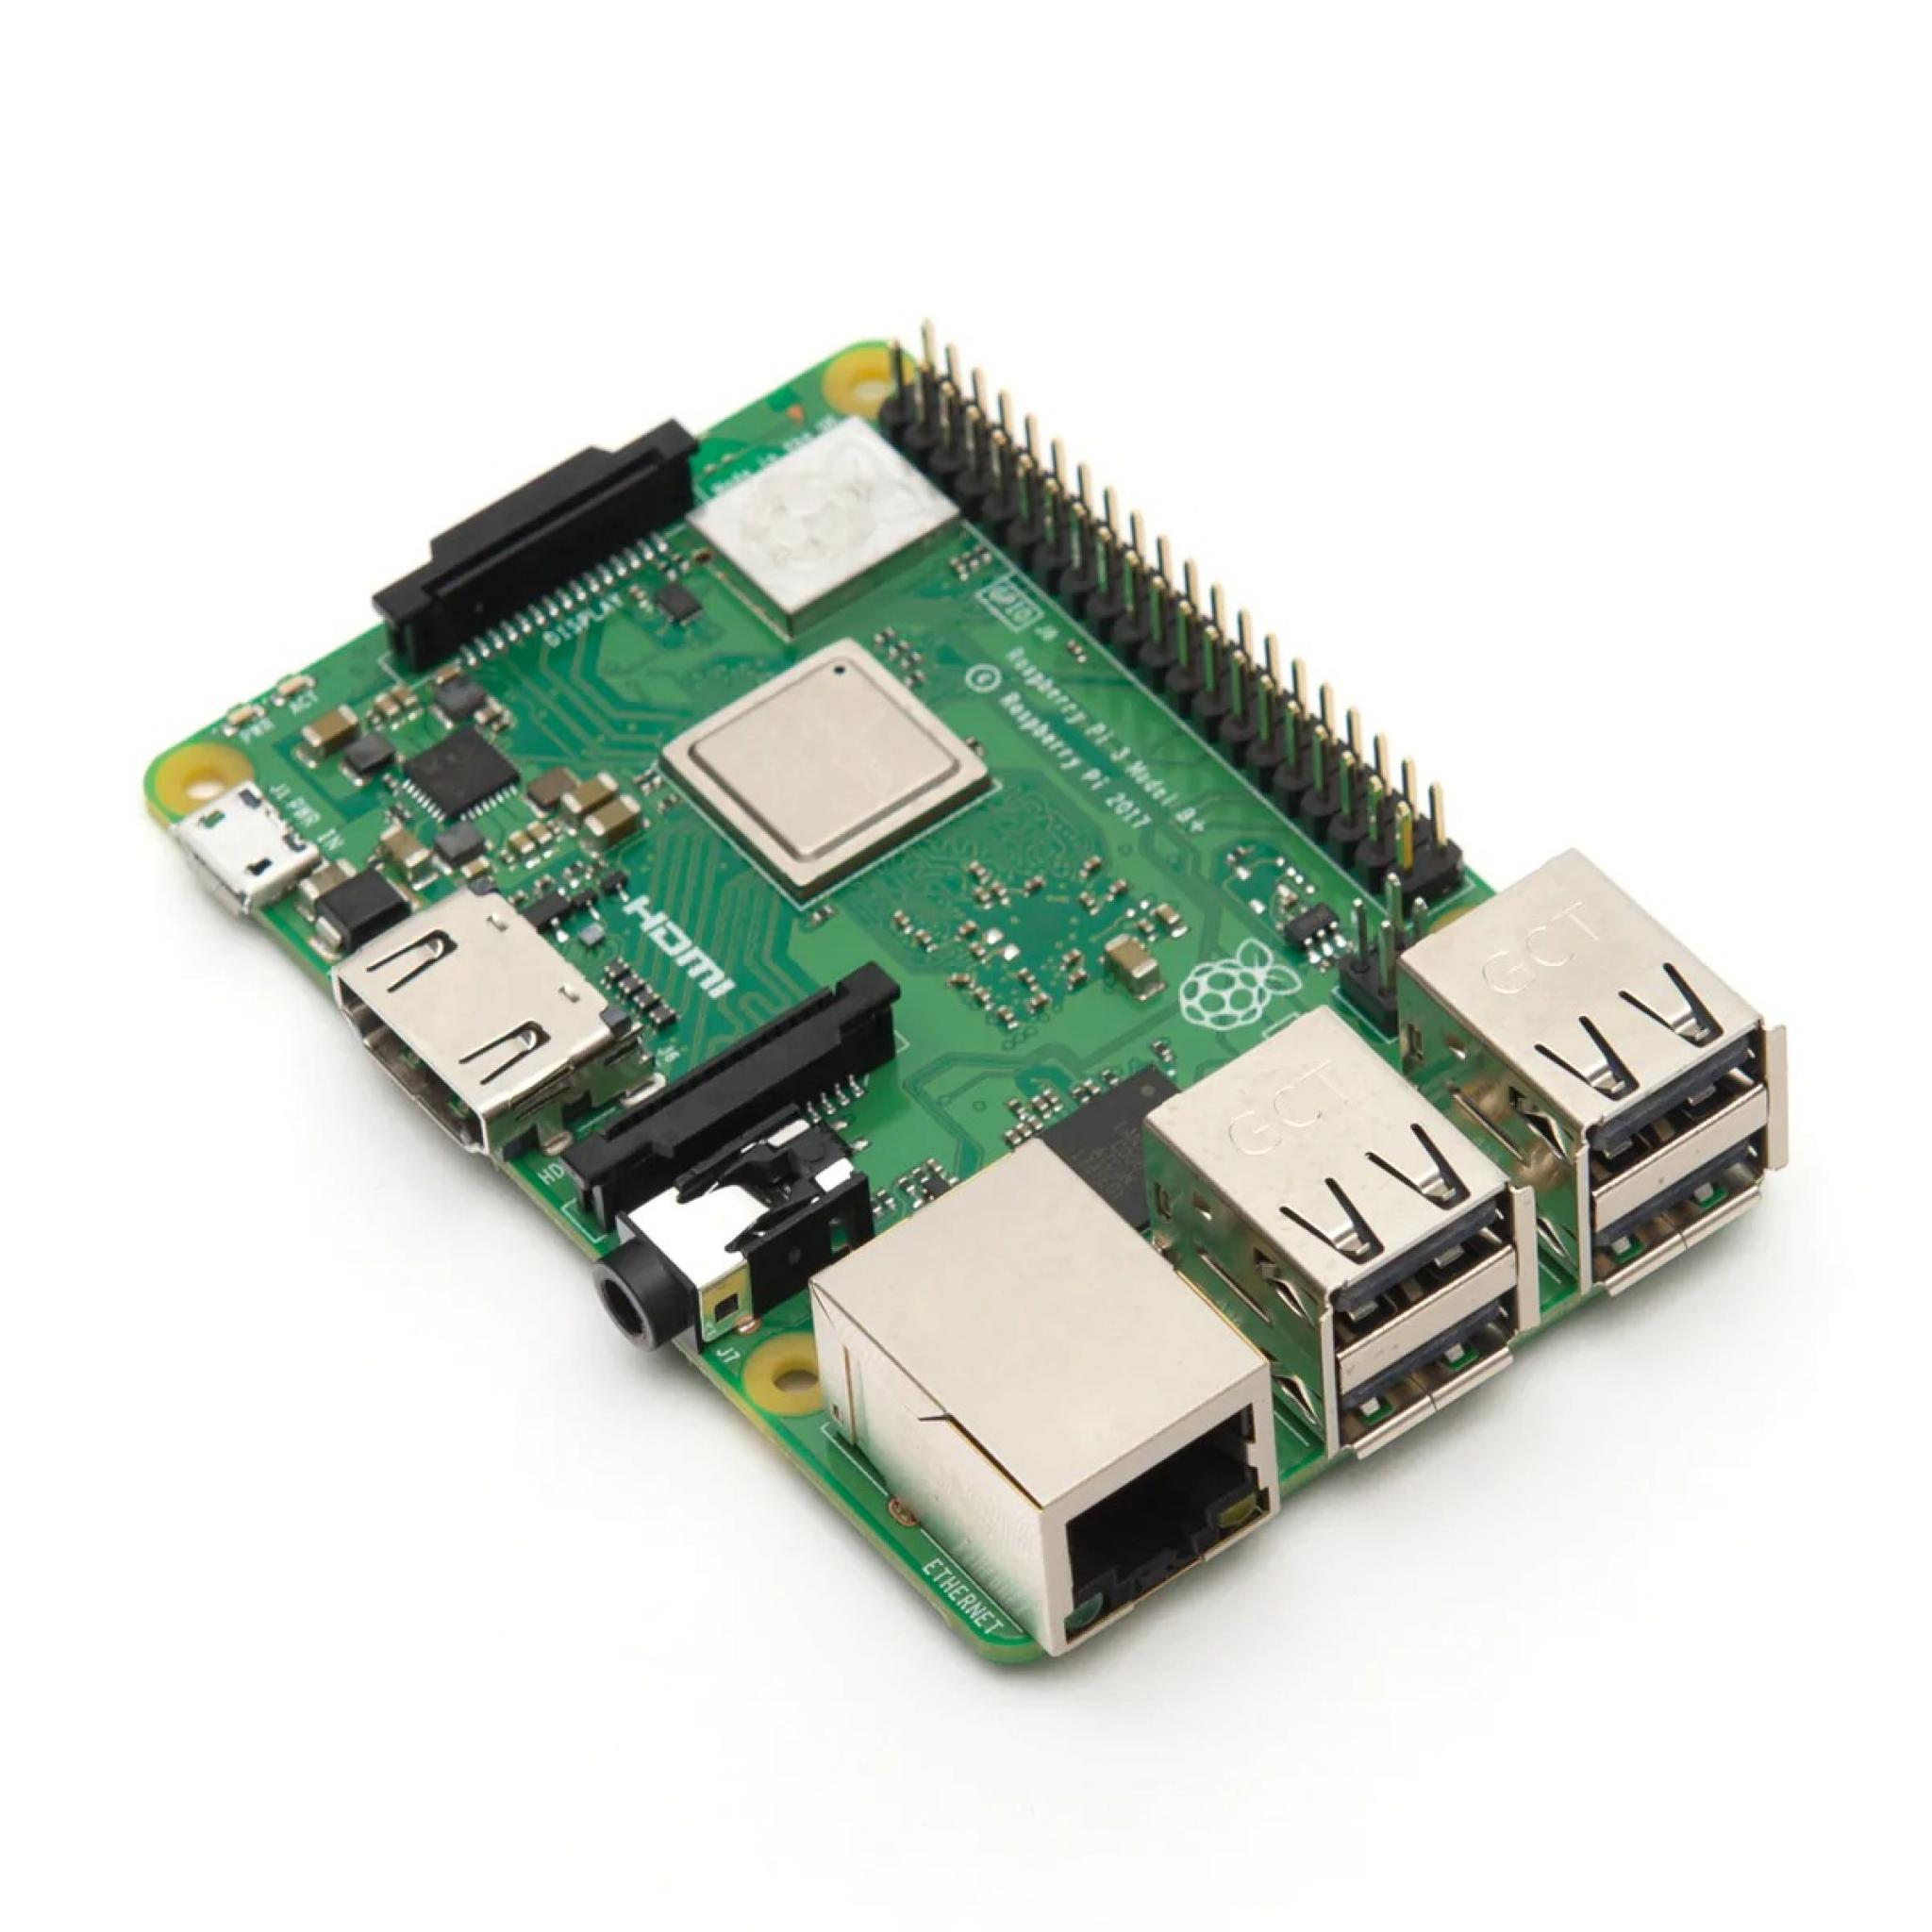
\includegraphics[width=0.4\textwidth]{imgs/Raspberry-pi3b+.jpg}
    \caption{Raspberry Pi 3B+.}
    \label{fig:raspberry}
\end{figure}

Otro de los puntos importantes que destacan de la placa son los pines GPIO, pines de entrada/salida de propósito general por sus siglas en inglés, lo que la hace sumamente sencilla a la hora de utilizarla junto a sensores comerciales.
La amplia conectividad integrada que posee fue un punto que la destacó sobre otras posibles placas de desarrollo, ya que cuenta con puertos de conexión USB 2.0, puerto Ethernet, conexión Wifi 2,4 y 5,8 GHz y comunicación Bluetooth 4.2, que suple la necesidad de brindar conexión a internet de manera nativa sin necesidad de contar con periféricos extras que pueden encarecer el sistema.

La disponibilidad de la placa en el mercado fue un punto importante a considerar, ya que se considera una futura implementación del sistema a mediana o gran escala o la necesidad de recambio por rotura. Por otro lado, este hardware permite migrar a un modelo más actual como la versión 4, sin tener que realizar grandes cambios en los drivers diseñados.


\subsection{Características del SL}

La placa del SL es una Nvidia Jetson TX1 \cite{nvidia_manual_nodate}, Fig. \ref{fig:JTX1} la cual cuenta con un procesador Cortex A57 y 4GB de RAM LPDDR4. Además contiene  256 núcleos Nvidia Maxwell, lo que la vuelve una opción excelente en lo que se refiere al trabajo con imágenes y videos.

Para realizar la implementación se contó con el kit de desarrollo provisto por la empresa Nvidia. En él se pueden encontrar todas las conexiones mencionadas en el SL mini, lo que permite el paso de los sensores de una placa a otra con suma facilidad.
Este modelo cuenta con un sistema operativo JetPack 4.6.3 basado en Ubuntu 18.04.

\begin{figure}[bth]
    \centering
    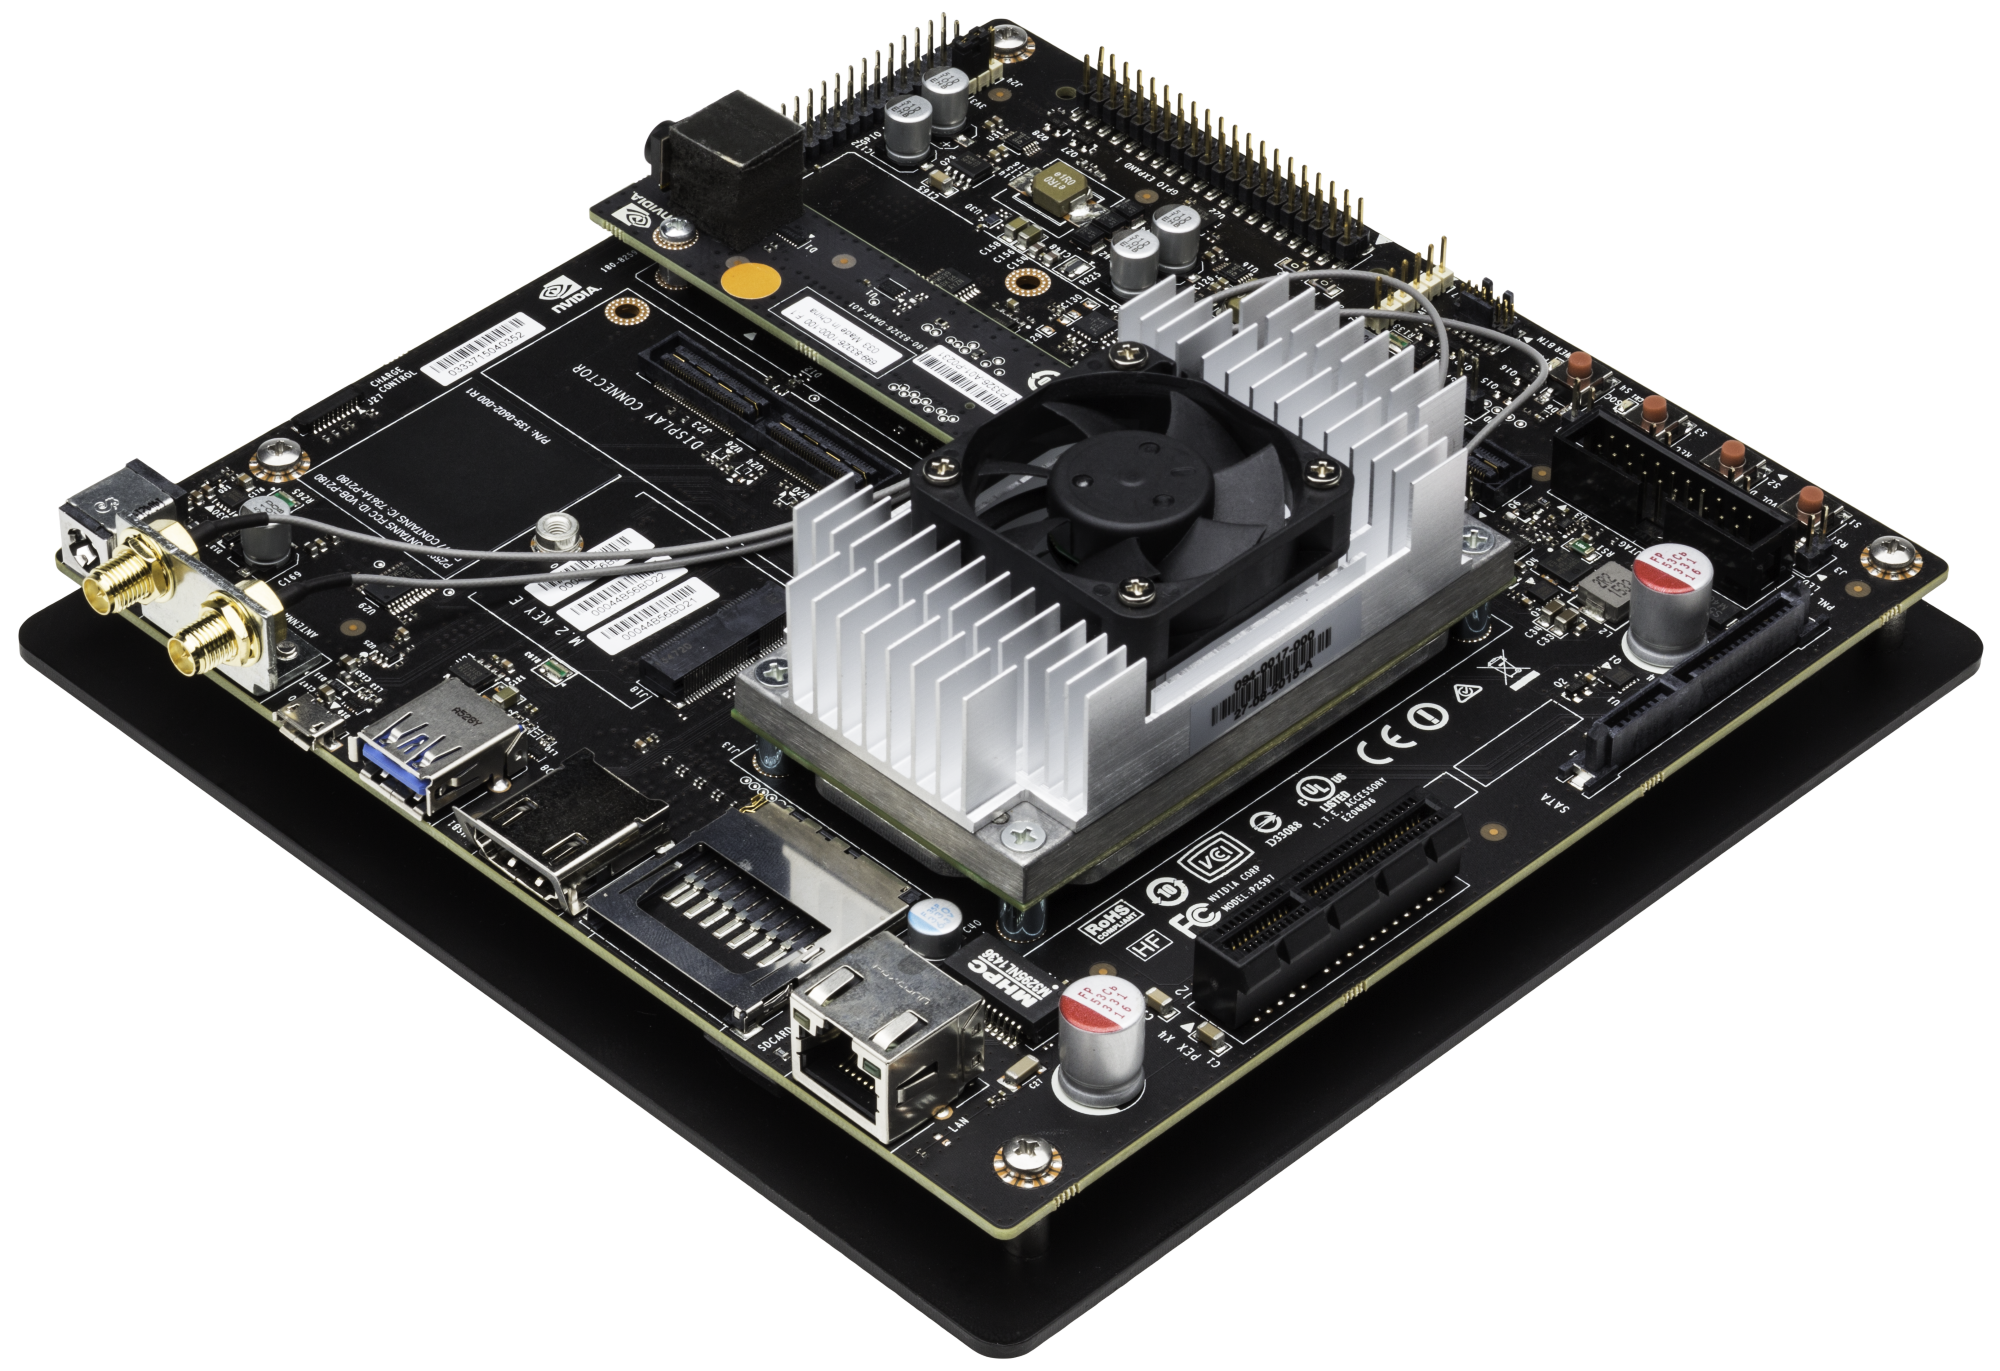
\includegraphics[width=0.3\textwidth]{imgs/JTX1-developerkit.png}
    \caption{Nvidia Jetson TX1 developer kit.}
    \label{fig:JTX1}
\end{figure}


En contra parte con el modelo mini, la placa del modelo SL está pensada para proyectos basados en redes neuronales y el procesamiento de imágenes, por lo que es posible integrar el algoritmo de OCR dentro del sistema, obteniendo un tiempo de respuesta de aproximadamente unos 6 segundos (Tab. \ref{tab:ocr}), tiempo que se consideró aceptable.


\begin{table}[bth]
    \centering
    \begin{tabular}{cccc}
        \toprule
        Módelo           & Cantidad de nucleos & RAM        & GPU        \\
        \midrule
        Raspberry Pi 3b+ & 4 a 1.4GHz          & 1GB LPDDR2 & 2 a 400MHz \\
        Jeston TX1       & 4 a                 & 4GB LPDDR4 & 256 a 1GHz \\
        \bottomrule
    \end{tabular}
    \caption{Resumen de características de las placas embebidas.}
\end{table}

\section{Evaluación y selección de sensores}

En este apartado se comentará la selección de la cámara y el proceso de selección del sistema de actuación que, como se adelantó en el capítulo 2, se decantó por un sensor de distancia.

\subsection{Selección de cámara}

Una cualidad importante para la selección del tipo de cámara fue la conexión, que permitiera implementar el mismo modelo en ambas versiones de placa.
Si bien, tanto Raspberry como NVIDIA proveen de módulos de cámara, debido a que los conectores no eran los mismos se descartaron estas opciones. La decisión final terminó siendo una cámara web con interfaz USB, debido a que hoy en día son fáciles de conseguir y son relativamente económicas. Particularmente el modelo utilizado es el que se observa en Fig. \ref{fig:camara-usb}, el cual es un modelo genérico con una resolución de $1280 \times 720$ y $0.9MP$, siendo estas características aceptables para la tarea requerida.

\begin{figure}[bth]
    \centering
    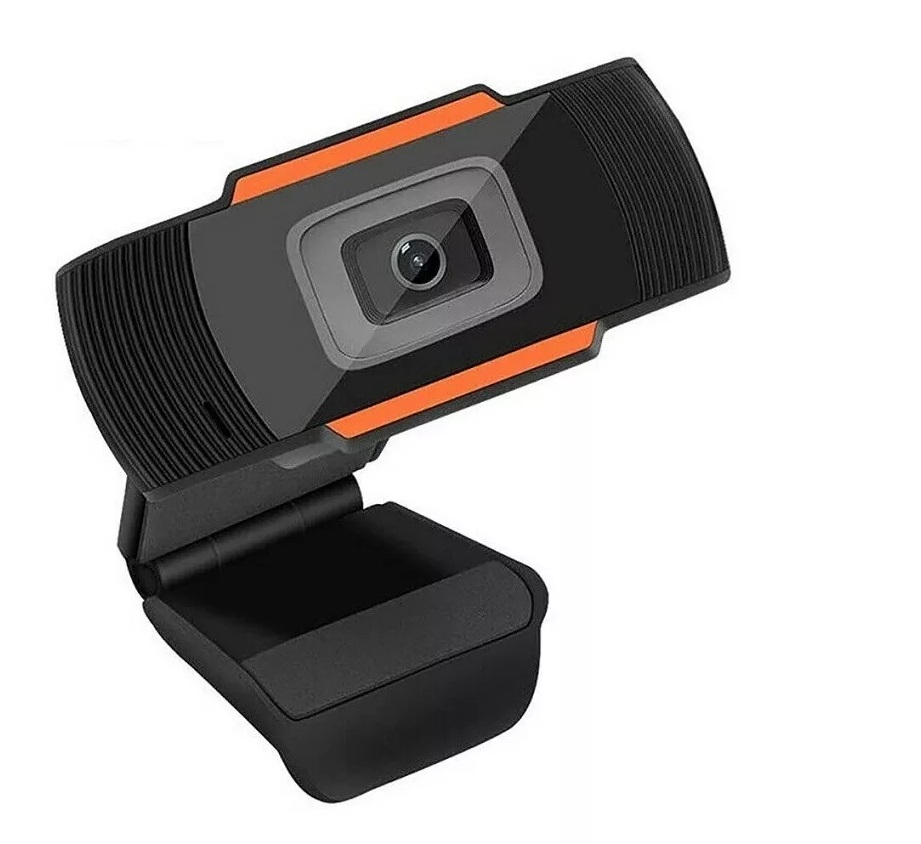
\includegraphics[width=0.4\textwidth]{imgs/camara-usb.jpg}
    \caption{Cámara utilizada.}
    \label{fig:camara-usb}
\end{figure}

\subsection{Selección de activador}

Con la finalidad de minimizar la captura de imágenes sin vehículos, se decidió colocar un sensor capaz de señalar que existe un objeto. A continuación se nombran las opciones analizadas:

\subsubsection{Barrera infrarroja}

Este sistema cuenta con un receptor y un emisor, separados lo suficiente para que un vehículo pase entre ellos. La captura se da cuando el vehículo interrumpe el paso de luz entre el receptor y el emisor.

El sistema de barrera infrarroja cuenta con una serie de inconvenientes que dificultan su implementación como:

\begin{enumerate}
    \item Potencia mínima para activar el receptor.
    \item Potencia máxima que puede emitir el trasmisor.
    \item Ruido producido por la luz ambiente u otras fuentes lumínicas.
    \item Apantallamiento del receptor debido a partículas de suciedad.
\end{enumerate}

\subsubsection{Placa de presión}

La placa de presión cuenta de un accionador que luego de ser pulsado activa el sistema. Debido a que no fue posible armar un sistema de placa a presión, y tampoco se consiguió una opción económicamente viable, sumado a que las dimensiones pueden variar dependiendo el estacionamiento esta opción fue descartada.

\subsubsection{Sensor de distancia}

Los sensores de distancia son muy versátiles y existen una amplia variedad en el mercado es por ello que fueron seleccionados para la implementación de los prototipos.
En particular para este trabajo se utilizó un sensor ultrasónico US-100.

Los sensores ultrasónicos funcionan emitiendo una onda ultrasónica por el transmisor y medir el tiempo que esta tarda en llegar al receptor.

El US-100 el cual se puede apreciar en Fig. \ref{fig:sensor-US100}, posee un rango de medición de $2cm$ a $350cm$, compensado por temperatura, voltaje de alimentación entre $3V$-$5V$ y protocolo de comunicación UART.
Por lo que es fácilmente integrable en ambas placas por medio del puerto GPIO sin necesidad de utilizar hardware extra.
\begin{figure}[bth]
    \centering
    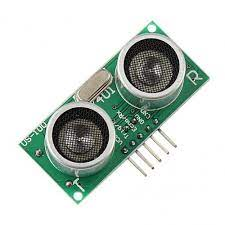
\includegraphics[width=0.3\textwidth]{imgs/us-100.jpg}
    \caption{Sensor de distancia ultrasónico US-100.}
    \label{fig:sensor-US100}
\end{figure}

\section{Consumo energético}

El gasto energético es un punto que fue analizado ya que, pensando en el uso racional de la energía, se busca que los sistemas SL y SL mini no presentaran un consumo excesivo.
Como la energía suministrada al conjunto cámara-sensor viene dada por las placas, solo se indicará el consumo requerido por las mismas.


\subsection{SL mini}

En el caso de la versión SL mini, tiene un consumo similar al de un cargador de celular moderno, es decir $5V$ y
$2A$.
Una corriente menor lleva a una notificación por parte de la Raspberry, lo que produce una reducción de la frecuencia de su procesador, una relentización del equipo, lo cual no garantiza estabilidad en el funcionamiento de la misma.

Por lo tanto la potencia máxima requerida del sistema es de $10W$.

\subsection{SL}

El requerimiento energético previsto por el fabricante para el kit de desarrollo de la Nvidia Jetson TX1 como se indica
en el cargador que viene dentro del kit es de $19V$ y $4.74A$, dando un máximo de $90W$, 9 veces mayor al del sistema SL mini.

\section{Diseño y ensamble}

Para la colocación del conjunto de prueba cámara-sensor, se diseñó e imprimió una caja en 3D, Fig. \ref{fig:contenedor-camara} que permita ser anclada a una pared o poste cercano a la zona de acceso. Este diseño permite una fácil instalación y puesta en marcha del sistema.
\begin{figure}[bth]
    \centering
    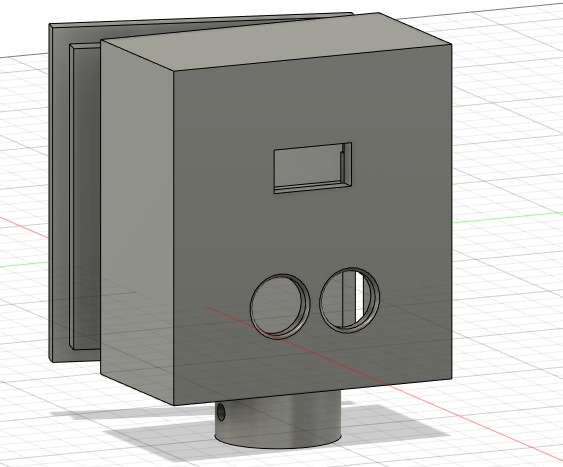
\includegraphics[width=0.5\textwidth]{imgs/contenedor-camara.png}
    \caption{Modelo 3D del contendor.}
    \label{fig:contenedor-camara}
\end{figure}

Se optó por colocar el sensor de proximidad en la zona inferior, ya que el ideal es colocar el contenedor a una altura de unos $60cm$ aproximadamente, con lo que al tener el sensor en la zona baja se garantiza que la lectura que se tome sea de la trompa del automóvil y se obtenga un valor certero de la distancia. Este diseño deja a la cámara en la zona superior del contendor dando una imagen lo más completa de la trompa del vehículo, lo que permite que el sistema reconozca la patente de mejor manera, esto previene que la patente salga recortada permitiendo mejores resultados en la etapa de estimación. Se dispuso un orificio en la zona inferior de la caja con la finalidad de colocar un eje, que permita la orientación del dispositivo, dependiendo
el lugar donde se desee instalarlo.
Para la sujeción al eje se realizaron dos orificios que permiten el paso de los tornillos que dejan fijo el contenedor al eje.
\begin{figure}[bth]
    \centering
    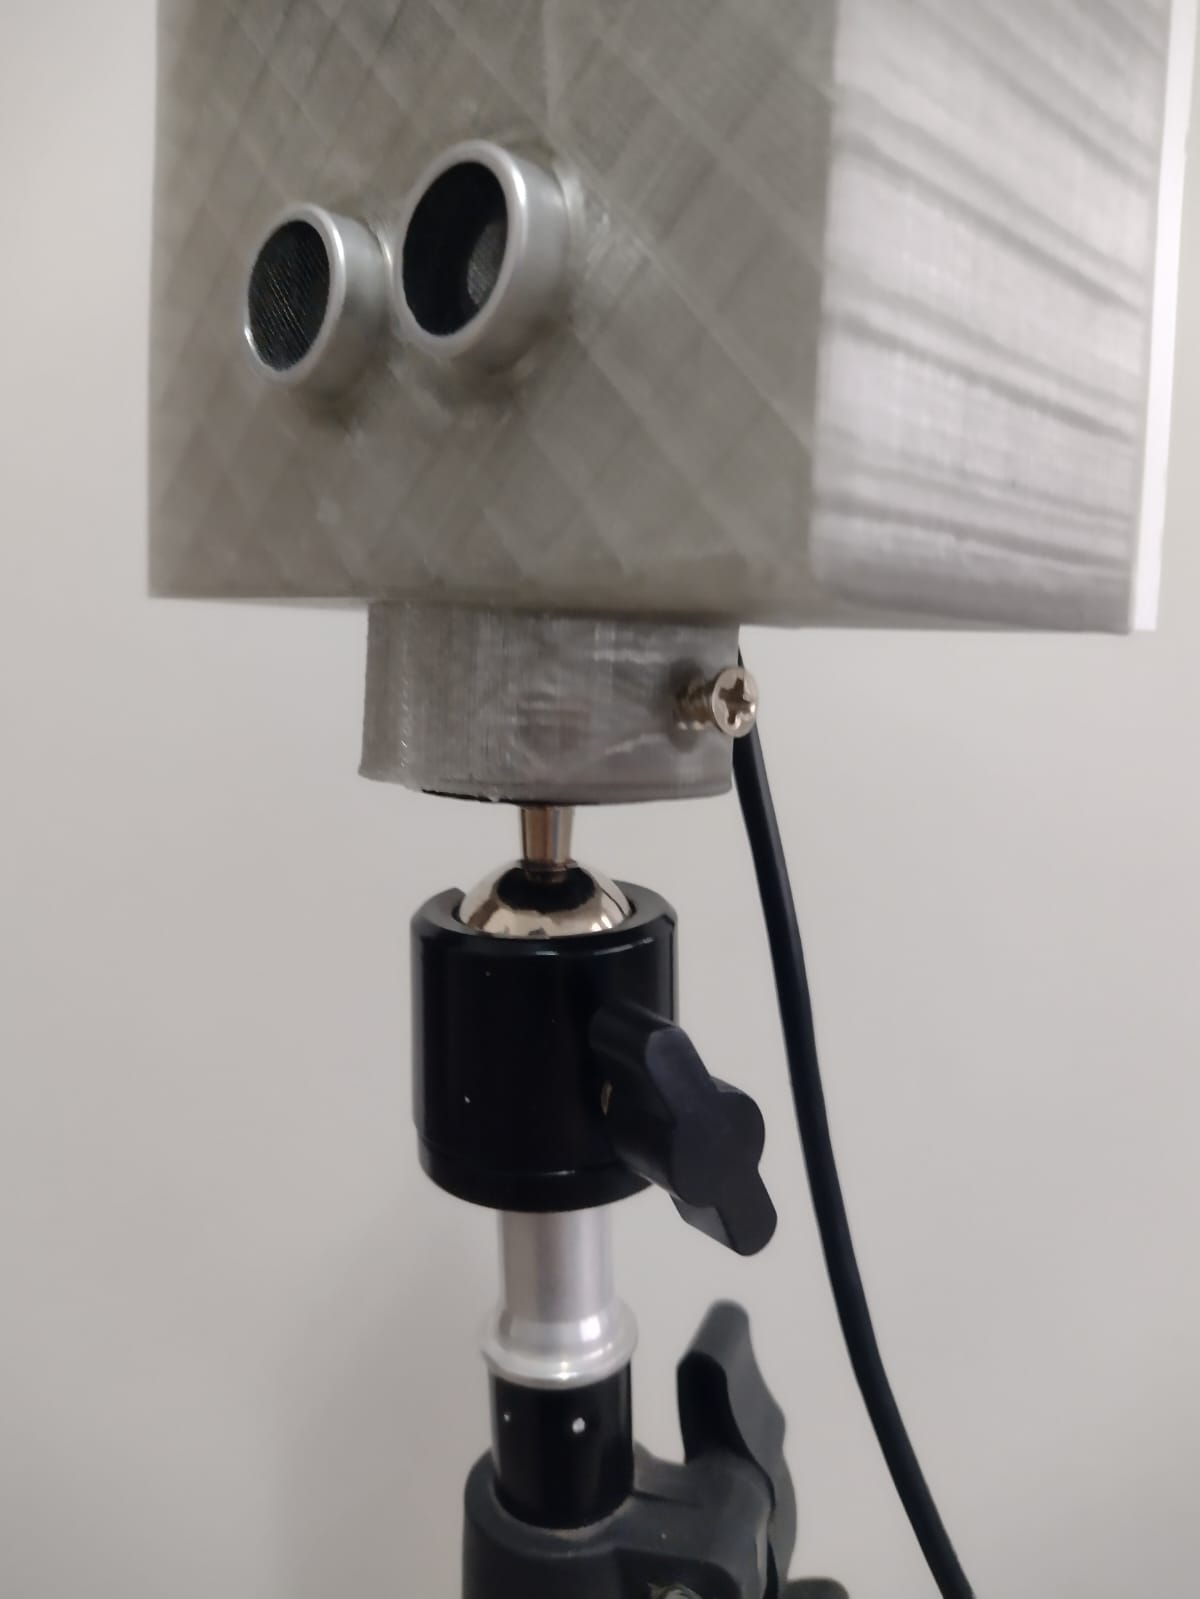
\includegraphics[width=0.5\textwidth]{imgs/sistema-sujecion.jpeg}
    \caption{Sistema de sujeción del contenedor.}
    \label{fig:sujecion-contenedor}
\end{figure}

En la Fig. \ref{fig:contenedor-camara-real} se puede apreciar el contenedor con la cámara y el sensor instalados.

\begin{figure}[bth]
    \centering
    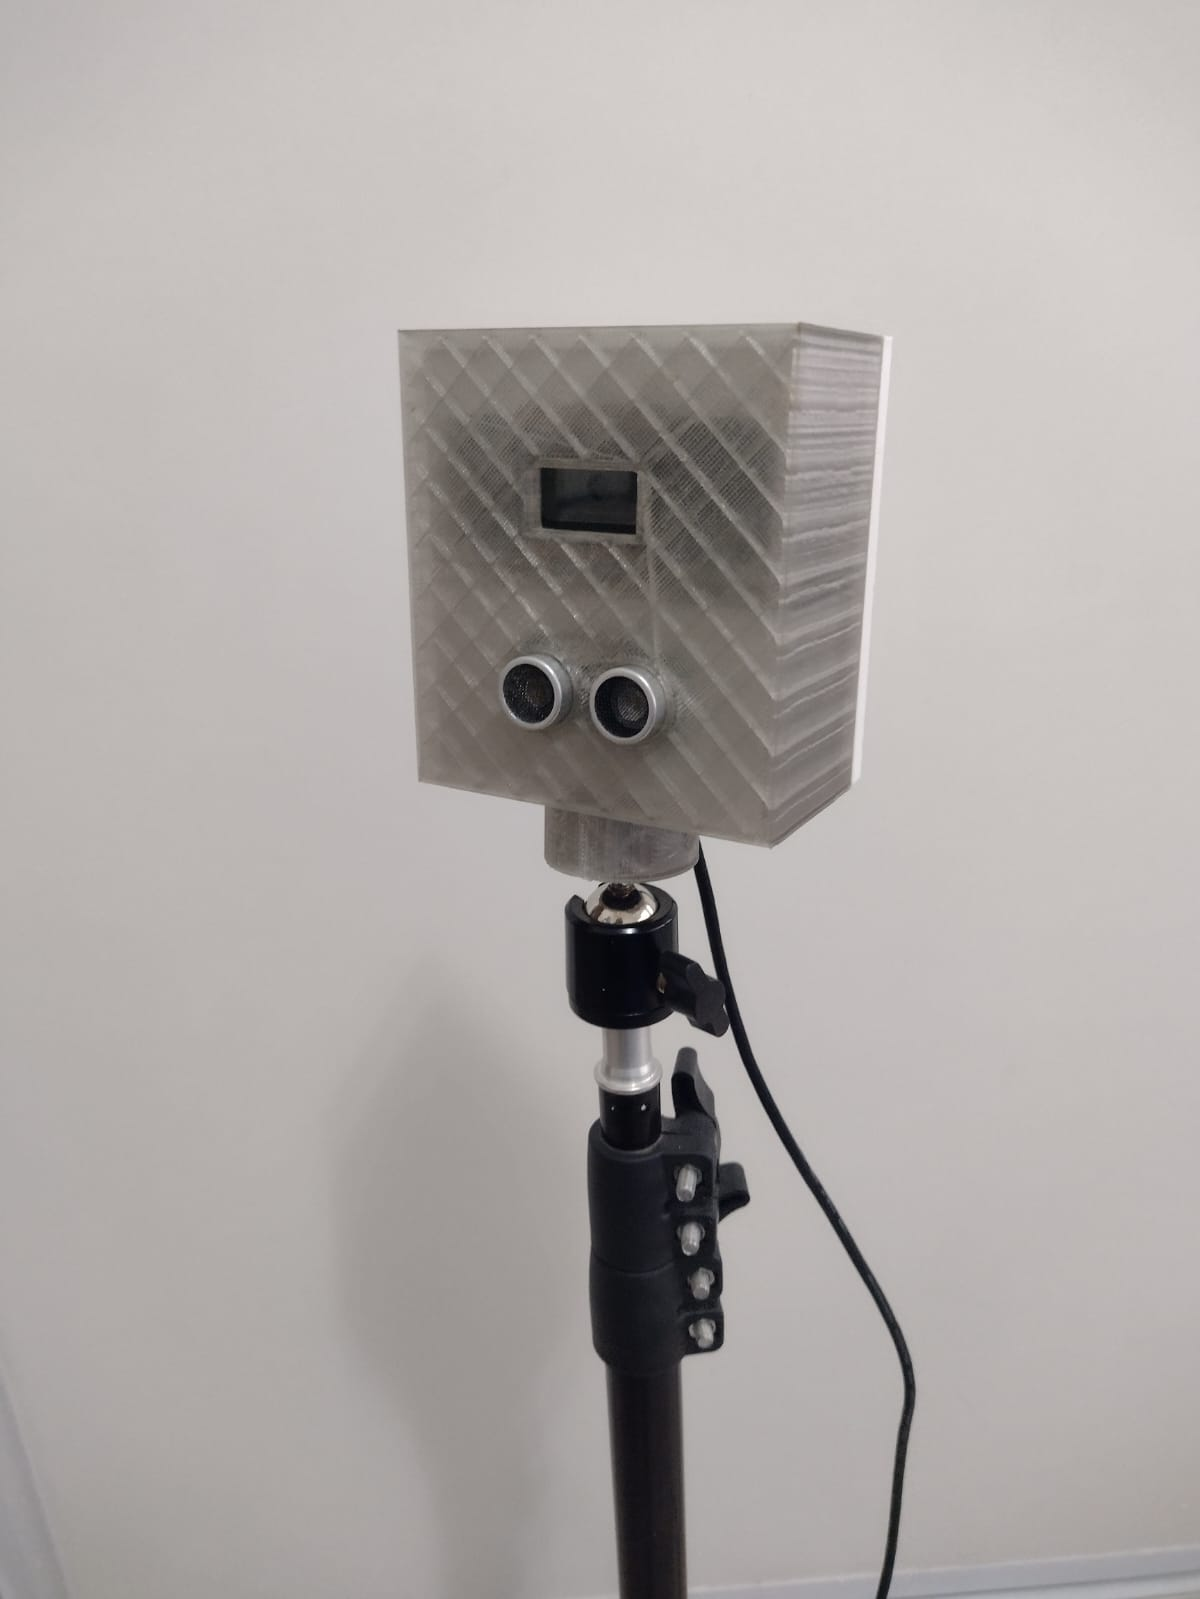
\includegraphics[width=0.5\textwidth]{imgs/contenedor-real.jpeg}
    \caption{Contendor del paquete cámara-sensor.}
    \label{fig:contenedor-camara-real}
\end{figure}

\section{Implementación de los drivers}

Para terminar el diseño de los sistemas SL y SL mini, se explicará el diseño de los drivers. Durante la etapa de diseño el eje fundamental fue crear piezas de códigos reutilizables, priorizando el diseño modular del sistema.
Es por ello que se implementaron una serie de módulos que permiten ser actualizados de manera sencilla y aíslan responsabilidades en diferentes partes. La implementación se realizó en Python 3. A continuación se realizará una breve explicación de las librerías creadas.


\subsubsection{Lectura de distancia}

Para la lectura de distancia se implementó una librería llamada \textit{us100}, la cual utiliza \textit{pyserial}  \cite{noauthor_documentacion_nodate-1} para la comunicación por puerto serie.
Esta librería posee una función que devuelve la distancia de un objetivo. Con la finalidad de disminuir los falsos positivos se utilizó una lista anidada que posee las últimas 5 mediciones, y devuelve el promedio de las mismas.

\subsubsection{Utilidades}

Se creó una librería llamada \textit{slutils} la cual tiene como responsabilidad la conexión con el servidor MQTT, el envío de registros de entrada/salida, así como administrar la configuración del sistema y la captura de imágenes.

Para la conexión con el servidor MQTT se utilizó \textit{paho-mqtt} \cite{craggs_documentacion_nodate}, escuchando el tópico \textit{$id/config$} donde el $id$ es un identificador único por cada placa.

En cuanto al envío de los registros este se realiza por POST mediante HTTP utilizando la librería \textit{requests} \cite{python_software_foundation_documentacion_nodate}.

La captura de imágenes se realizó mediante la librería de \textit{OpenCV}, que permite una fácil conexión con la cámara USB logrando tomar fotografías rápidamente.

\subsection{Diferencias entre SL y SL mini}

Como fue nombrado con anterioridad, la mayor diferencia entre ambos sistemas es que el sistema SL es capaz de procesar la imagen de manera local. Esto implica que una conversión de los modelos de Tensorflow \cite{google_tensorflow_nodate} utilizados para la CNN-OCR a una versión capaz de correr en ARM, por lo que se compilaron los modelos a Tensorflow Lite, utilizando las herramientas que Tensorflow provee para estos casos. Por otro lado, se requiere compilar la YoloV4 para arquitectura ARM, esto se realizó utilizando el compilador de CMake.

